\documentclass[12pt]{amsart}
% packages
\usepackage{graphicx}
\usepackage{setspace}
\usepackage{amssymb,amsmath,amsthm,amsfonts,amscd}
\usepackage{hyperref}
\usepackage{color}
\usepackage{booktabs}
\usepackage{tabularx}
\usepackage{enumitem}
\usepackage[retainorgcmds]{IEEEtrantools}
\usepackage[notref,notcite,final]{showkeys}
\usepackage[final]{pdfpages}
\usepackage{fancyhdr}
\usepackage{upgreek}
\usepackage{multicol}
\usepackage{fontawesome}
\usepackage{halloweenmath}
% set margin as 0.75in
\usepackage[margin=0.75in]{geometry}

% tikz-related settings
\usepackage{tkz-berge}
\usetikzlibrary{calc,quotes}
\usetikzlibrary{arrows.meta}
\usetikzlibrary{positioning, automata}
\usetikzlibrary{decorations.pathreplacing}

%% For table
\usepackage{tikz}
\usetikzlibrary{tikzmark}

% theorem environments with italic font
\newtheorem{thm}{Theorem}[section]
\newtheorem*{thm*}{Theorem}
\newtheorem{lemma}[thm]{Lemma}
\newtheorem{prop}[thm]{Proposition}
\newtheorem{claim}[thm]{Claim}
\newtheorem{corollary}[thm]{Corollary}
\newtheorem{conjecture}[thm]{Conjecture}
\newtheorem{question}[thm]{Question}
\newtheorem{procedure}[thm]{Procedure}
\newtheorem{assumption}[thm]{Assumption}

% theorem environments with roman font (use lower-case version in body
% of text, e.g., \begin{example} rather than \begin{Example})
\newtheorem{Definition}[thm]{Definition}
\newenvironment{definition}
{\begin{Definition}\rm}{\end{Definition}}
\newtheorem{Example}[thm]{Example}
\newenvironment{example}
{\begin{Example}\rm}{\end{Example}}

\theoremstyle{definition}
\newtheorem{remark}[thm]{\textbf{Remark}}

% special sets
\newcommand{\A}{\mathbb{A}}
\newcommand{\C}{\mathbb{C}}
\newcommand{\F}{\mathbb{F}}
\newcommand{\N}{\mathbb{N}}
\newcommand{\Q}{\mathbb{Q}}
\newcommand{\R}{\mathbb{R}}
\newcommand{\Z}{\mathbb{Z}}
\newcommand{\cals}{\mathcal{S}}
\newcommand{\ZZ}{\mathbb{Z}_{\ge 0}}
\newcommand{\cala}{\mathcal{A}}
\newcommand{\calb}{\mathcal{B}}
\newcommand{\cald}{\mathcal{D}}
\newcommand{\calh}{\mathcal{H}}
\newcommand{\call}{\mathcal{L}}
\newcommand{\calr}{\mathcal{R}}
\newcommand{\la}{\mathbf{a}}
\newcommand{\lgl}{\mathfrak{gl}}
\newcommand{\lsl}{\mathfrak{sl}}
\newcommand{\lieg}{\mathfrak{g}}

% math operators
\DeclareMathOperator{\kernel}{\mathrm{ker}}
\DeclareMathOperator{\image}{\mathrm{im}}
\DeclareMathOperator{\rad}{\mathrm{rad}}
\DeclareMathOperator{\id}{\mathrm{id}}
\DeclareMathOperator{\hum}{[\mathrm{Hum}]}
\DeclareMathOperator{\eh}{[\mathrm{EH}]}
\DeclareMathOperator{\lcm}{\mathrm{lcm}}
\DeclareMathOperator{\Aut}{\mathrm{Aut}}
\DeclareMathOperator{\Inn}{\mathrm{Inn}}
\DeclareMathOperator{\Out}{\mathrm{Out}}
\DeclareMathOperator{\Gal}{\mathrm{Gal}}


% frequently used shorthands
\newcommand{\ra}{\rightarrow}
\newcommand{\se}{\subseteq}
\newcommand{\ip}[1]{\langle#1\rangle}
\newcommand{\dual}{^*}
\newcommand{\inverse}{^{-1}}
\newcommand{\norm}[2]{\|#1\|_{#2}}
\newcommand{\abs}[1]{\lvert #1 \rvert}
\newcommand{\Abs}[1]{\bigg| #1 \bigg|}
\newcommand\bm[1]{\begin{bmatrix}#1\end{bmatrix}}
\newcommand{\op}{\text{op}}

% nicer looking empty set
\let\oldemptyset\emptyset
\let\emptyset\varnothing

%the var phi gang
\let\oldphi\phi
\let\phi\varphi

\setlist[enumerate,1]{topsep=1em,leftmargin=1.8em, itemsep=0.5em, label=\textup{(}\arabic*\textup{)}}
\setlist[enumerate,2]{topsep=0.5em,leftmargin=3em, itemsep=0.3em}

%pagestyle
%\pagestyle{fancy} 

\begin{document}
\begin{center}
    \textsc{Math 605B. HW 4\\ Ian Jorquera}
\end{center}
\vspace{1em}

% https://www.omnicalculator.com/math/chinese-remainder
\begin{itemize}
\item[(2)]
\iffalse
E = EllipticCurve([0, 1])
K.<a> = E.division_field(3)
EK = E.change_ring(K); EK
T = EK.torsion_subgroup(); 
TT= [T[t] for t in range(0, 36) if T[0]==3*T[t]]; TT

# This gives the 3-torsion points where a is a root of x^6 + 3*x^5 + 6*x^4 + 15*x^3 + 18*x^2 - 9*x + 9
#[T[0],T[2],T[4],T[12],T[14],T[16],T[24],T[26],T[28]]
#EK
#x = PolynomialRing(ComplexField(), 'x').gen()
#f = x^6 + 3*x^5 + 6*x^4 + 15*x^3 + 18*x^2 - 9*x + 9
#f.factor()
\fi

Here to compute the $3$-torsion points of $E:y^2=x^3+1$ we can us the following sage code that first finds the smallest field in which all $3$-torsion points exist. This is the field $\Q[\alpha]$ where $\alpha$ is a root of the polynomial $x^6 + 3x^5 + 6x^4 + 15x^3 + 18x^2 - 9x + 9$. The sage code used is 

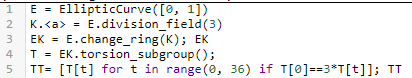
\includegraphics[]{pics/hw4sage1ag.png}

And the $3$-torsion points are

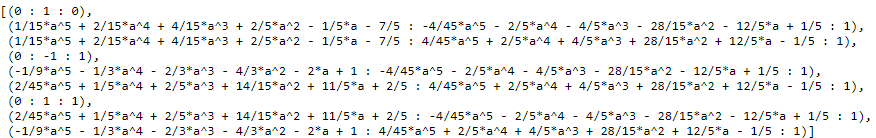
\includegraphics[scale=.95]{pics/hw4sage2ag.png}\\

We can explicitly compute the value of $\alpha\approx 0.2937 - 2.2408i$ in the complex number using sage.


\item[(3)] 
\iffalse
E = EllipticCurve('11a'); E
#K.<a> = E.division_field(5)
#EK = E.change_ring(K); EK
#T = EK.torsion_subgroup(); T
T = E.torsion_subgroup(); T
TT= [T[t] for t in range(0, 5) if T[0]==5*T[t]]; TT
\fi

Sage defaults to giving the elliptical curve in Weierstrass form: $y^2 + y = x^3 - x^2 - 10x - 20$. To get it in a shorter form we can use the short\_weierstrass\_model fuction and get that $y^2 = x^3 - 13392x - 1080432$ 

Now to find the points of order $5$, which we can compute in the same way as before to find the $5$-torsion points, this time we will focus only on the rational $5$-torsion points. We can follow the same process as before 

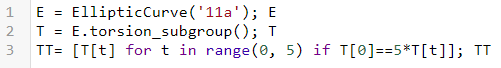
\includegraphics[]{pics/hw4sage3ag.png}

Where we find the following rational torsion points

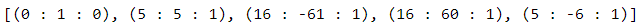
\includegraphics[]{pics/hw4sage4ag.png}\\

\item[(7)] Notice that $F(X,Y,Z)$ has the following partial derivatives: $F_X(X,Y,Z)=3X^2$, $F_Y(X,Y,Z)=3Y^2$, and $F_X(X,Y,Z)=-3AZ^2$. Notice that for all partials to be zero we would have $[0:0:0]$ which is not valid point in $\mathbb{P}^2$. So $E$ is smooth. Notice that when $Z=0$ we have that $X^3=-Y^3$ which is the case when $P_\infty=[-1:1:0]$. With sage we can determine that when $A=1$, in Weierstrass form this is $y^2+9y=x^3-27$ and with sage we can compute the $j$-invariant to be $j=0$ when $A=1$. We only need to consider the case of $A= 1$ as any value of $A$ gives an isomorphic elliptical curve up to rescaling of $Z$.\\
% E = EllipticCurve([0, 1])
%G = E.torsion_subgroup(); G
%G.gen(0);
%[3*E(t) for t in G];

%var('A')
%R.<x,y,z>= QQ[]; F = x^3+y^3-A*z^3; P = [1,-1,0];
%E = EllipticCurve(F,P); E

\item [(8)] Consider a point $P=[x_0:y_0:z_0]$ on the elliptical curve $E$. To find $-P$ we know that the points $P$, $-P$ and $P_\infty$ are colinear. So we can compute the line containing $P$ and $P_\infty$. That is we have the line $\alpha x+\beta y + \gamma z = 0$ knowing $P_\infty=[1:-1:0]$ is a point on this line we have that $\alpha-\beta=0$ meaning $\alpha=\beta$. So the line is of the form $\alpha x + \alpha y +\gamma z =0$ which is symmetric in $x$ and $y$. And because the elliptical curve $e:x^3+y^3-Az^3=0$ is also symmetric in $x$ and $y$ we know that the point $[x_0:y_0:z_0]$ lives on the line if and only if $[y_0:x_0:z_0]$ lives on the line. So $-P=[y_0:x_0:z_0]$.\\

Now we want to compute $2P$. Notice that the line tangent to $P$ on the elliptical curve must intersect the elliptical curve at a point $R$ such that $P+P+R=0$, meaning $2P=-R$. To construct the line tangent to the curve we can use the partial derivatives which gives us the line $x_0^2x+y_0^2y-Az_0^2z=0$ after rescaling common factors. Now we want to show that $R$ lives on this line where $-R=[-y_0(x_0^3+Az_0^3):x_0(y_0^3+Az_0^3):x_0^3z_0-y_0^3z_0]$ which it does and we may also show that $R$ lives on the elliptical curve. And so $2P=-R$. 

\end{itemize}

\end{document}






